\DocumentMetadata{
 lang=en,
 pdfversion=2.0,
 pdfstandard=ua-2,
 pdfstandard=a-4f, % needs to be remove so Canvas Ally accepts title
 tagging=on,
 tagging-setup={math/setup=mathml-SE},
 debug={xmp-export}
}

% !TEX root = Syllabus_Accessibility.tex
\documentclass[12pt,letterpaper]{article}
% basic style definitions for lecture notes in text mode.
% based on material from J. W. Langelaan, August 16, 2010

% Vitor T. Valente, August 2024
\DocumentMetadata{
  tagging = on,
  lang = en,
  pdfstandard = ua-2,
  pdfstandard = a-4f, % optional archival standard
  tagging-setup = {math/setup={mathml-AF,mathml-SE},
                   extra-modules={verbatim-mo},
                   table/header-rows=1}}

\documentclass[times,12pt,letterpaper]{article}

\usepackage{latexsym}
\usepackage{fancyhdr}
\usepackage{amsmath, amsthm}
\usepackage{amsfonts}
\usepackage{amssymb}
\usepackage{amsxtra}
\usepackage{graphicx}
\usepackage{epstopdf}
 \usepackage{subfigure}			% subcaptions for subfigures
 \usepackage{subfigmat}			% matrices of similar subfigures, aka small mulitples
\usepackage{times}
\usepackage[small]{caption}
\usepackage{wrapfig}			% wrap figures/tables in text (i.e., Di Vinci style)
\usepackage{color}
\usepackage{ifthen}
\usepackage{float}
\usepackage{multicol}
\usepackage[normalem]{ulem}
\usepackage{titling}
\usepackage{url}
\usepackage{hyperref}


\usepackage{tikz} % For block diagrams
\usetikzlibrary{positioning}

\usepackage{times}
\usepackage{unicode-math}

\newcommand{\myheading}[1]
	{\noindent \textbf{#1}}

\newcommand{\mat}[1]  % define command for bold upright matrix notation (also gives bold greek)
    {\mbox{\boldmath$\mathrm{#1}$}}

\newcommand{\ddt}[1] {\frac{d{#1}}{dt}}
\newcommand{\deldel}[2]{\frac{\delta {#1}}{\delta {#2}}}
\newcommand{\DEG}[1] {\mbox{${#1}^{\circ}$}}
\newcommand{\LAPL}[1]{\mathcal{L}\left\{{#1}\right\}}
\newcommand{\iLAPL}[1]{\mathcal{L}^{-1}\left\{{#1}\right\}}

\pagestyle{fancy}

\newcommand{\course}[1]{\lhead{\textbf{ \footnotesize{#1}}}}
\chead{}
\newcommand{\lecture}[1]{\rhead{\textbf{\footnotesize{#1--\thepage}}}}
\newcommand{\semester}[1]{\lfoot{\textbf{\footnotesize{#1}}}}
\cfoot{}
\rfoot{\textbf{}}
\renewcommand{\headrulewidth}{0pt}
\renewcommand{\footrulewidth}{0pt}

\newcommand{\printnotes}{\printnotestrue}

% Prevent word splitting (hyphenation) and penalize it if it occurs
\hyphenpenalty=10000
\exhyphenpenalty=10000
\sloppy

% define an environment that prints out notes to self in red if \printnotes is true, in white (on white paper,
% hence invisible) otherwise. Printing notes in white will leave space for student notes...
\newif\ifprintnotes
\newenvironment{mynotes}
{
	\ifprintnotes
		\color{red}
	\else
		\color{white}
	\fi
}
{
	\color{black}
}

\definecolor{codegreen}{rgb}{0,0.6,0}
\definecolor{codegray}{rgb}{0.5,0.5,0.5}
\definecolor{codepurple}{rgb}{0.58,0,0.82}
\definecolor{backcolorPython}{rgb}{0.90,0.95,0.92}
\definecolor{backcolorMatlab}{rgb}{0.95,0.90,0.92}
\definecolor{backcolorCpp}{rgb}{0.95,0.95,0.90}


\printnotestrue % set to true to print notes in red,
% \printnotesfalse % set to false to hide notes (white on white paper)

% ======= INIT =========
\begin{document}

\begin{center}
    \huge Introduction to Dynamics and Control\par
    \normalsize AERSP 304 - Dynamics and Control of Aerospace Systems\par
    \bigskip
    \bigskip
    \normalsize V.T. Valente\par
    \small Penn State University\par
    \normalsize January 14, 2026
\end{center}

\bigskip
\noindent The goals for today lecture are to:\par
\begin{itemize}
    \setlength{\itemsep}{0.0cm}
    \setlength{\parsep}{0cm}
    \item Review the definition of Frame of References
    \item Review the definition of DCMs
    \item Review time derivatives of vectors in different frames of reference
\end{itemize}

\bigskip
\section*{Reference Frames}
\indent A \emph{frame} is a language used to convey dynamical information. A frame is a coordinate system defined by an origin and a set of basis vectors. It is used to describe the position, orientation, and motion of objects in space. Different frames can be used to describe the same physical situation from different perspectives.\par\smallskip
A dynamical information example is the orientation of a rigid body in space, which can be described using a body-fixed frame and an inertial frame. Position and velocity are other examples of dynamical information that can be conveyed using frames of reference.\par\smallskip

\begin{mynotesfigures}

\tagstructbegin{tag=Figure, alttext={3D coordinate system}}
\begin{center}
    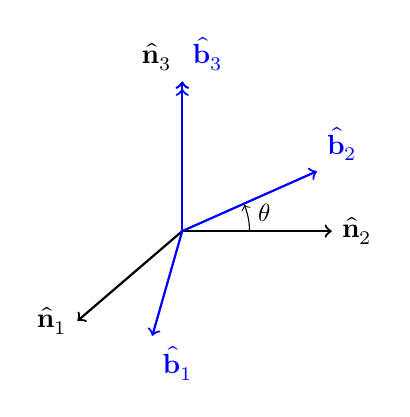
\begin{tikzpicture}[scale=0.95, line cap=round, line join=round]
        % origin
        \coordinate (O) at (0,0);

        % inertial (N) axes
        \draw[->, thick] (O) -- (-1.4,-1.2) node[left]  {$\hat{\mathbf n}_1$};
        \draw[->, thick] (O) -- ( 2.0, 0.0) node[right] {$\hat{\mathbf n}_2$};
        \draw[->, thick] (O) -- ( 0.0, 2.0) node[above left] {$\hat{\mathbf n}_3$};

        % body (B) axes
        \draw[->, thick, blue] (O) -- ( -0.4,-1.4) node[below right] {$\hat{\mathbf b}_1$};
        \draw[->, thick, blue] (O) -- ( 1.8, 0.8) node[above right] {$\hat{\mathbf b}_2$};
        \draw[->>, thick, blue] (O) -- ( 0.0, 2.0) node[above right] {$\hat{\mathbf b}_3$};

        % angle between b2 and n2
        \draw[->] (0.9,0.0) arc[start angle=0, end angle=23, radius=0.9];
        \node at (1.1,0.25) {\small$\theta$};
    \end{tikzpicture}
\end{center}
\tagstructend
\end{mynotesfigures}

\normalsize
\begin{mynotes}
Frame $N$: $\left\{0, \hat{\mathbf n}_1, \hat{\mathbf n}_2, \hat{\mathbf n}_3 \right\}$ and Frame $B$: $\left\{0, \hat{\mathbf b}_1, \hat{\mathbf b}_2, \hat{\mathbf b}_3 \right\}$\par

\medskip

Frame $N$ is said to be orthonormal and dextral (right-handed) if its basis vectors satisfy:
\[
    \hat{\mathbf n}_1 \times \hat{\mathbf n}_2 = \hat{\mathbf n}_3
\]
\end{mynotes}

\subsection*{Frame Orientation}
\indent How is the $B$ oriented w.r.t. the frame $N$?\par

\medskip
We are looking for a language translator to express the basis vectors of frame $B$ in terms of the basis vectors of frame $N$. This language translator is called the Direction Cosine Matrix (DCM) and is denoted, in this case, by $C_{BN}$.\par\smallskip
But before we jump into the DCMs, let's first understand how to express the coordinates of a vector in frame $B$ in terms of the coordinates of the same vector in frame $N$. We want to find a relationship (which physical quantity is that?) between the coordinates of a vector expressed in frame $N$ and frame $B$. \par\medskip

\begin{mynotes}
    We have the information of frame $N$. We know how its basis vectors are oriented in space. We want to express the basis vectors of frame $B$ in terms of the basis vectors of frame $N$.
    \par\smallskip
    In other words, if dealing only with unit vectors:
    \[
        \hat{\mathbf b}_1 = ( \qquad )\,\hat{\mathbf n}_1 + ( \qquad )\,\hat{\mathbf n}_2 + ( \qquad )\,\hat{\mathbf n}_3
    \]
    \medskip
    Let's look at the 2D sketch of the frames again to get some intuition.
    \par\smallskip
    \tagstructbegin{tag=Figure, alttext={3D coordinate system}}
    \begin{center}
        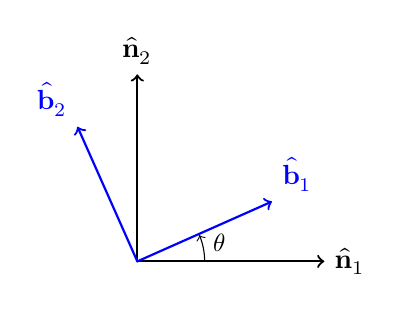
\begin{tikzpicture}[scale=0.95, line cap=round, line join=round]
               % origin
                \coordinate (O) at (0,0);
                % inertial (N) axes
                \draw[->, thick, black] (O) -- ( 2.5, 0.0) node[right]  {$\hat{\mathbf n}_1$};
                \draw[->, thick, black] (O) -- ( 0.0, 2.5) node[above] {$\hat{\mathbf n}_2$};
                % body (B) axes
                \draw[->, thick, blue] (O) -- ( 1.8, 0.8) node[above right] {$\hat{\mathbf b}_1$};
                \draw[->, thick, blue] (O) -- ( -0.8, 1.8) node[above left] {$\hat{\mathbf b}_2$};
                % angle between b1 and n1
                \draw[->, black] (0.9,0.0) arc[start angle=0, end angle=23, radius=0.9];
                \node[black] at (1.1,0.25) {\small$\theta$};
        \end{tikzpicture}
    \end{center}
    \tagstructend
    \par\smallskip
    From the sketch, we can see that:
    \[
        \hat{\mathbf b}_1 = \cos\theta\,\hat{\mathbf n}_1 + \sin\theta\,\hat{\mathbf n}_2
    \]
    \[
        \hat{\mathbf b}_2 = -\sin\theta\,\hat{\mathbf n}_1 + \cos\theta\,\hat{\mathbf n}_2
    \]
    \par\smallskip
    From there, we conclude that the physical quantity that relates the coordinates of a vector expressed in frame $N$ to the coordinates of the same vector expressed in frame $B$ is build on the projection of $\hat{\mathbf b}_i$ onto $\hat{\mathbf n}_j$.
    \par\medskip
    The mathematical representation of a projection is the dot product:
    \[
        \hat{\mathbf b}_1 \cdot \hat{\mathbf n}_1 = | \hat{\mathbf b}_1 |\,| \hat{\mathbf n}_1 |\,\cos\theta = \cos\theta
    \]
\end{mynotes}

\subsection*{Direction Cosine Matrix}
\indent The Direction Cosine Matrix (DCM) is a matrix that describes the orientation of one frame relative to another. It is constructed using the dot products of the basis vectors of the two frames. The DCM maps coordinates from frame $N$ to frame $B$ and is denoted by $C_{BN}$.\par\smallskip

Let $\hat{\mathbf r}$ be a vector expressed in frame $N$ as:
\[
    \hat{\mathbf r} = x_N\,\hat{\mathbf n}_1 + y_N\,\hat{\mathbf n}_2 + z_N\,\hat{\mathbf n}_3
\]
and in frame $B$ as:
\[
    \hat{\mathbf r} = x_B\,\hat{\mathbf b}_1 + y_B\,\hat{\mathbf b}_2 + z_B\,\hat{\mathbf b}_3
\]
\par\smallskip
To find the relationship between the coordinates in frame $B$ and frame $N$, we can take the dot product of both sides of the equation with each of the basis vectors of frame $B$.
\par\smallskip
\begin{mynotes}
    Taking the dot product with $\hat{\mathbf b}_1$:
    \[
        \hat{\mathbf r} \cdot \hat{\mathbf b}_1 = x_B\,(\hat{\mathbf b}_1 \cdot \hat{\mathbf b}_1) + y_B\,(\hat{\mathbf b}_2 \cdot \hat{\mathbf b}_1) + z_B\,(\hat{\mathbf b}_3 \cdot \hat{\mathbf b}_1)
    \]
    \[
        \hat{\mathbf r} \cdot \hat{\mathbf b}_1 = x_B
    \]
    since the basis vectors are orthonormal.\par\smallskip
    Similarly, taking the dot product with $\hat{\mathbf b}_2$ and $\hat{\mathbf b}_3$ gives:
    \[
        \hat{\mathbf r} \cdot \hat{\mathbf b}_2 = y_B
    \]
    \[
        \hat{\mathbf r} \cdot \hat{\mathbf b}_3 = z_B
    \]
    \par\smallskip
    Now, substituting the expression for $\hat{\mathbf r}$ in terms of frame $N$ into these equations, we get:
    \[
        x_B = x_N\,(\hat{\mathbf n}_1 \cdot \hat{\mathbf b}_1) + y_N\,(\hat{\mathbf n}_2 \cdot \hat{\mathbf b}_1) + z_N\,(\hat{\mathbf n}_3 \cdot \hat{\mathbf b}_1)
    \]
    \[
        y_B = x_N\,(\hat{\mathbf n}_1 \cdot \hat{\mathbf b}_2) + y_N\,(\hat{\mathbf n}_2 \cdot \hat{\mathbf b}_2) + z_N\,(\hat{\mathbf n}_3 \cdot \hat{\mathbf b}_2)
    \]
    \smallskip
    \[
        z_B = x_N\,(\hat{\mathbf n}_1 \cdot \hat{\mathbf b}_3) + y_N\,(\hat{\mathbf n}_2 \cdot \hat{\mathbf b}_3) + z_N\,(\hat{\mathbf n}_3 \cdot \hat{\mathbf b}_3)
    \]
\end{mynotes}

\medskip
The result is the following matrix equation:
\[
    \begin{bmatrix}
        x_B\\[0.2em]
        y_B\\[0.2em]
        z_B
    \end{bmatrix}
    =
    \underbrace{\begin{bmatrix}
        \hat{\mathbf b}_1\!\cdot\!\hat{\mathbf n}_1 & \hat{\mathbf b}_1\!\cdot\!\hat{\mathbf n}_2 & \hat{\mathbf b}_1\!\cdot\!\hat{\mathbf n}_3\\
        \hat{\mathbf b}_2\!\cdot\!\hat{\mathbf n}_1 & \hat{\mathbf b}_2\!\cdot\!\hat{\mathbf n}_2 & \hat{\mathbf b}_2\!\cdot\!\hat{\mathbf n}_3\\
        \hat{\mathbf b}_3\!\cdot\!\hat{\mathbf n}_1 & \hat{\mathbf b}_3\!\cdot\!\hat{\mathbf n}_2 & \hat{\mathbf b}_3\!\cdot\!\hat{\mathbf n}_3
    \end{bmatrix}}_{C_{BN}}
    \begin{bmatrix}
        x_N\\[0.2em]
        y_N\\[0.2em]
        z_N
    \end{bmatrix}
\]

The matrix $C_{BN}$ is the Direction Cosine Matrix (DCM) that maps coordinates from frame $N$ to frame $B$.\par\smallskip

What is the orientation of frame $N$ w.r.t. frame $B$? The answer is given by the inverse of the DCM:
\[
    \begin{bmatrix}
        x_N\\[0.2em]
        y_N\\[0.2em]
        z_N
    \end{bmatrix}
    =
    C_{NB}
    \begin{bmatrix}
        x_B\\[0.2em]
        y_B\\[0.2em]
        z_B
    \end{bmatrix},
    \quad
    \text{where} \quad
    C_{NB} = \left(C_{BN}\right)^{-1}.
\]\par\smallskip

Since DCMs are orthogonal matrices, their inverse is equal to their transpose:
\[
    C_{NB} = \left(C_{BN}\right)^{T}.
\]

Let's now consider another frame $A$ rotating w.r.t. frame $B$. What is the orientation of the frame $A$ w.r.t. frame $N$?\par\smallskip

The DCM that maps coordinates from frame $N$ to frame $A$ is given by the product of the DCMs that map coordinates from frame $N$ to frame $B$ and from frame $B$ to frame $A$:

\begin{mynotes}
    \[
        \begin{bmatrix}
            x_A\\[0.2em]
            y_A\\[0.2em]
            z_A
        \end{bmatrix}
        =
        C_{AN}
        \begin{bmatrix}
            x_N\\[0.2em]
            y_N\\[0.2em]
            z_N
        \end{bmatrix},
        \quad
        \text{where} \quad
        C_{AN} = C_{AB} \, C_{BN}.
    \]

    The notation starts at the rightmost subindex and goes to the leftmost subindex. We want to go to the left from $N$ to $A$, so we first go from $N$ to $B$ and then from $B$ to $A$. \par\bigskip
\end{mynotes}

\subsection*{Independent Parameters}
Let a DCM be defined by the following elements:
\[
    C =
    \begin{bmatrix}
        C_{11} & C_{12} & C_{13}\\
        C_{21} & C_{22} & C_{23}\\
        C_{31} & C_{32} & C_{33}
    \end{bmatrix}
\]

Since DCMs are orthogonal matrices, they satisfy the following properties:
\[
    C^{T} C = C C^{T} = I
\]
where $I$ is the identity matrix. This leads to the following constraints on the elements of the DCM:
\[
    C_{11}^2 + C_{21}^2 + C_{31}^2 = 1
\]
\[
    C_{12}^2 + C_{22}^2 + C_{32}^2 = 1
\]
\[
    C_{13}^2 + C_{23}^2 + C_{33}^2 = 1
\]
\[
    C_{11} C_{12} + C_{21} C_{22} + C_{31} C_{32} = 0
\]
\[
    C_{11} C_{13} + C_{21} C_{23} + C_{31} C_{33} = 0
\]
\[
    C_{12} C_{13} + C_{22} C_{23} + C_{32} C_{33} = 0
\]

\par\smallskip

These relations can also be achieved by trying to project a frame in itself and knowing that the dot product of orthonormal basis vectors is either 1 (if the vectors are the same) or 0 (if the vectors are different):\par\smallskip
\[
    \hat{\mathbf b}_1 = (\hat{\mathbf b}_1 \cdot \hat{\mathbf b}_1)\,\hat{\mathbf b}_1 + (\hat{\mathbf b}_2 \cdot \hat{\mathbf b}_1)\,\hat{\mathbf b}_2 + (\hat{\mathbf b}_3 \cdot \hat{\mathbf b}_1)\,\hat{\mathbf b}_3
\]
\[
    \hat{\mathbf b}_2 = (\hat{\mathbf b}_1 \cdot \hat{\mathbf b}_2)\,\hat{\mathbf b}_1 + (\hat{\mathbf b}_2 \cdot \hat{\mathbf b}_2)\,\hat{\mathbf b}_2 + (\hat{\mathbf b}_3 \cdot \hat{\mathbf b}_2)\,\hat{\mathbf b}_3
\]
\[
    \hat{\mathbf b}_3 = (\hat{\mathbf b}_1 \cdot \hat{\mathbf b}_3)\,\hat{\mathbf b}_1 + (\hat{\mathbf b}_2 \cdot \hat{\mathbf b}_3)\,\hat{\mathbf b}_2 + (\hat{\mathbf b}_3 \cdot \hat{\mathbf b}_3)\,\hat{\mathbf b}_3
\]

\par\smallskip
That means:\par\smallskip
\[
    \hat{\mathbf b}_1 \cdot \hat{\mathbf b}_1 = 1, \quad \hat{\mathbf b}_2 \cdot \hat{\mathbf b}_2 = 1, \quad \hat{\mathbf b}_3 \cdot \hat{\mathbf b}_3 = 1
\]
\[
    \hat{\mathbf b}_1 \cdot \hat{\mathbf b}_2 = 0, \quad \hat{\mathbf b}_1 \cdot \hat{\mathbf b}_3 = 0, \quad \hat{\mathbf b}_2 \cdot \hat{\mathbf b}_3 = 0
\]

So, in conclusion, the total number of independent parameters to define a DCM is 3. A common representation of a DCM is given by the use of Euler angles, which are three angles that describe the orientation of a rigid body with respect to a fixed coordinate system.

\subsubsection*{Euler Angles}
Euler angles are a set of three angles that describe the orientation of a rigid body in three-dimensional space. They are commonly used in aerospace engineering to represent the orientation of aircraft and spacecraft. The three Euler angles are typically denoted as roll ($\phi$), pitch ($\theta$), and yaw ($\psi$).\par\smallskip

The Euler Theorem states that any orientation of a rigid body can be achieved by a sequence of three rotations about the axes of a coordinate system. The most common sequence of rotations is the Z-Y-X sequence.\par\smallskip

Let a position vector $\bar{\mathbf r}_p$ be defined as:

\begin{mynotes}
\[
    \bar{\mathbf r}_p = x\,\hat{\mathbf n}_1 + y\,\hat{\mathbf n}_2 + z\,\hat{\mathbf n}_3
\]

Or simply $\left[ \bar{\mathbf r}_p \right]_N$. The representation in the body frame is given by $\left[ \bar{\mathbf r}_p \right]_B$:

\[
    \left[ \bar{\mathbf r}_p \right]_B = C_{BN} \, \left[ \bar{\mathbf r}_p \right]_N
\]

Here, $\bar{\mathbf r}_p$ is the information we are trying to describe and the frames $N$ and $B$ are the languages we are using to describe it. Therefore, the position vector can have different expressions that represent the same information:

\[
    \left[ \bar{\mathbf r}_p \right]_N = ( \qquad )\,\hat{\mathbf n}_1 + ( \qquad )\,\hat{\mathbf n}_2 + ( \qquad )\,\hat{\mathbf n}_3
\]
\[
    \left[ \bar{\mathbf r}_p \right]_B = ( \qquad )\,\hat{\mathbf b}_1 + ( \qquad )\,\hat{\mathbf b}_2 + ( \qquad )\,\hat{\mathbf b}_3
\]
\end{mynotes}


\section*{Time Derivative of a Vector in Different Frames}

Let's first look at the time derivative of a vector expressed in a single frame of reference. Considering a 2D case:\par\smallskip
\begin{mynotesfigures}

    \tagstructbegin{tag=Figure, alttext={2D coordinate system}}
    \begin{center}
        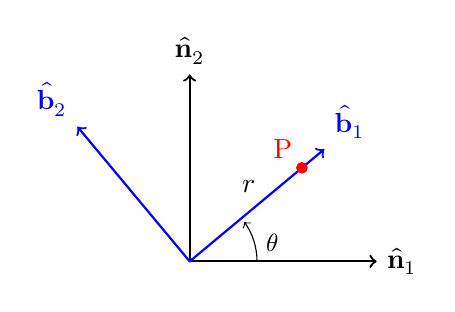
\begin{tikzpicture}[scale=0.95, line cap=round, line join=round]
            % origin
             \coordinate (O) at (0,0);
             % inertial (N) axes
             \draw[->, thick, black] (O) -- ( 2.5, 0.0) node[right]  {$\hat{\mathbf n}_1$};
             \draw[->, thick, black] (O) -- ( 0.0, 2.5) node[above] {$\hat{\mathbf n}_2$};
             % body (B) axes
             \draw[->, thick, blue] (O) -- ( 1.8, 1.5) node[above right] {$\hat{\mathbf b}_1$};
             \draw[->, thick, blue] (O) -- ( -1.5, 1.8) node[above left] {$\hat{\mathbf b}_2$};
             % angle between b1 and n1
             \draw[->, black] (0.9,0.0) arc[start angle=0, end angle=36, radius=0.9];
             \node[black] at (1.1,0.25) {\small$\theta$};
             % add point P
             \filldraw[red] (1.5,1.25) circle (2pt) node[above left] {P};
             \node at (1.0,1.0) [left] {$r$};
     \end{tikzpicture}
    \end{center}
    \tagstructend
\end{mynotesfigures}

\begin{mynotes}

The position vector of point P can be defined in two different ways, depending on the frame of reference used:
\[
    \bar{\mathbf r} = r\,\hat{{\mathbf b}}_1
\]
or
\[
    \bar{\mathbf r} = r\,\cos\theta\,\hat{{\mathbf n}}_1 + r\,\sin\theta\,\hat{{\mathbf n}}_2
\]

If we consider the observer to be in the body frame $B$, the time derivative of the position vector, in the $B$ frame is given by:
\[
    {}^{B}\dot{\bar{\mathbf r}}  = \dot{r}\,\hat{{\mathbf b}}_1
\]
However, if the observer, then we will be defining the time derivative of the position vector in the $B$ frame, or inertial velocity in the $B$ frame, as given by:
\[
    {}^{N}\dot{\bar{\mathbf r}} = \dot{r}\,\hat{{\mathbf b}}_1 + r\,\dot{\hat{{\mathbf b}}}_1 = {}^{N}\dot{\bar{\mathbf r}}_{B}
\]
At this point, we need to find $\dot{\hat{{\mathbf b}}}_1$. For that we will use the Transport Theorem.\par\medskip
\end{mynotes}

\subsection*{Transport Theorem}
\indent The Transport Theorem relates the time derivative of a vector as observed in two different frames of reference. It states that the time derivative of a vector $\hat{\mathbf b}_1$ in frame $N$ is equal to the time derivative of the vector in frame $B$ plus the cross product of the angular velocity of frame $B$ relative to frame $N$ and the vector $\hat{\mathbf b}_1$ itself:

\[
    \boxed{
    {}^{N}\dot{\hat{\mathbf b}}_1 = {}^{B}\dot{\hat{\mathbf b}}_1 + \bar{\boldsymbol{\omega}}_{B/N} \times \hat{\mathbf b}_1
    }
\]

However, the frame $B$ is fixed, so the time derivative of its basis vectors in its own frame is zero. Therefore:
\[
    {}^{N}\dot{\hat{\mathbf b}}_1 = \bar{\boldsymbol{\omega}}_{B/N} \times \hat{\mathbf b}_1
\]

The term $\bar{\boldsymbol{\omega}}_{B/N}$ is directly the angular velocity of frame $B$ w.r.t. frame $N$.\par\smallskip
Substituting this result back into the expression for the time derivative of the position vector in frame $N$, we get:
\[
    {}^{N}\dot{\bar{\mathbf r}} = \dot{r}\,\hat{{\mathbf b}}_1 + r\,\dot{\hat{{\mathbf b}}}_1
\]
\[
    {}^{N}\dot{\bar{\mathbf r}} = \dot{r}\,\hat{{\mathbf b}}_1 + r\,\left( \bar{\boldsymbol{\omega}}_{B/N} \times \hat{\mathbf b}_1 \right)
\]

The term ${}^{N}\dot{\bar{\mathbf r}}$ is the inertial velocity and can be expressed in any frame of reference.\par\medskip

The angular velocity vector $\bar{\boldsymbol{\omega}}_{B/N}$ is perpendicular to the plane formed by $\hat{\mathbf b}_1$ and $\hat{\mathbf b}_2$. Therefore, its direction is along the axis $\hat{\mathbf b}_3$ (out of the page) and its magnitude is given by $\dot{\theta}$:
\[
    \bar{\boldsymbol{\omega}}_{B/N} = \dot{\theta}\,\hat{\mathbf b}_3
\]
\par\smallskip
Now, we can compute the cross product:
\[
    \dot{\hat{{\mathbf b}}}_1 = \dot{\theta}\,\hat{\mathbf b}_3 \times \hat{\mathbf b}_1 = \dot{\theta}\,\hat{\mathbf b}_2
\]
\par\smallskip
Substituting this result back into the expression for the time derivative of the position vector, for an observer in frame $N$ and expressed in the $B$ frame, we get:
\[
    {}^{N}\dot{\bar{\mathbf r}} = \dot{r}\,\hat{{\mathbf b}}_1 + r\,\dot{\theta}\,\hat{\mathbf b}_2
\]

% Now consider that a third frame $A$ is rotating w.r.t. frame $N$. What is the time derivative of a vector expressed in frame $A$ as observed in frame $N$?\par\smallskip

% \begin{mynotes}
% Now consider the case where there is a single rotation between frames $N$ and $A$.

% \begin{mynotesfigures}
% \tagstructbegin{tag=Figure, alttext={2D coordinate system}}
% \begin{center}
%     \begin{tikzpicture}[scale=0.95, line cap=round, line join=round]
%         % origin
%         \coordinate (O) at (0,0);
%         % inertial (N) axes
%         \draw[->, thick, black] (O) -- ( 2.5, 0.0) node[right]  {$\hat{\mathbf n}_1$};
%         \draw[->, thick, black] (O) -- ( 0.0, 2.5) node[above] {$\hat{\mathbf n}_2$};
%         % body (B) axes
%         \draw[->, thick, blue] (O) -- ( 1.8, 1.5) node[above right] {$\hat{\mathbf b}_1$};
%         \draw[->, thick, blue] (O) -- ( -1.5, 1.8) node[above left] {$\hat{\mathbf b}_2$};
%         % body (A) axes
%         \draw[->, thick, green] (O) -- ( 2.8, 1.0) node[above right] {$\hat{\mathbf a}_1$};
%         % angle between b1 and n1
%         \draw[->,black] (0.9,0.0) arc[start angle=0, end angle=36, radius=0.9];
%         \node[black] at (1.1,0.25) {\small$\theta$};
%         % angle between b1 and a1
%         \draw[->,black] (1.8,0.0) arc[start angle=0, end angle=32, radius=0.9];
%         \node[black] at (2.0,0.25) {\small$\phi$};
%         % add point P
%         \filldraw[red] (1.5,1.25) circle (2pt) node[above left] {P};
%         \node at (1.0,1.0) [left] {$r$};
%     \end{tikzpicture}
% \end{center}
% \tagstructend
% \end{mynotesfigures}

% In order to find the time derivative of $\hat{\mathbf a}_1$, we need to compute the angular velocity of frame $A$ w.r.t. frame $N$, $\bar{\boldsymbol{\omega}}_{A/N}$. Since there is only a single rotation between frames $N$ and $A$, the angular velocity vector is perpendicular to the plane formed by $\hat{\mathbf a}_1$ and $\hat{\mathbf a}_2$. Therefore, its direction is along the axis $\hat{\mathbf a}_3$ (out of the page) and its magnitude is given by $\dot{\phi}$:

% \[
%     \bar{\boldsymbol{\omega}}_{A/N} = \dot{\phi}\,\hat{\mathbf a}_3
% \]

% Using the Transport Theorem, we can express the time derivative of $\hat{\mathbf a}_1$ in frame $N$ as:
% \[
%     {}^{N}\dot{\hat{\mathbf a}}_1 = {}^{A}\dot{\hat{\mathbf a}}_1 + \bar{\boldsymbol{\omega}}_{A/N} \times \hat{\mathbf a}_1
% \]

% Assuming now that both frames are rotating, we can also express the point $P$ in terms of frame $A$, from an observer in frame $A$ by using the Transport Theorem and the difference in angular velocity between frames $A$ and $B$.

% \[
%     \bar{\boldsymbol{\omega}}_{A/B} = \dot{\theta}\,\hat{\mathbf b}_3 - \dot{\phi}\,\hat{\mathbf a}_3
% \]

% Since frame $A$ and frame $B$ are both aligned, the axis of rotation is the same. Therefore, we can simplify the previous expression considering that $\hat{\mathbf b}_3 = \hat{\mathbf a}_3$.\par\bigskip
% \end{mynotes}

Let's now consider the 3D general case:\par\smallskip
\tagstructbegin{tag=Figure, alttext={3D coordinate system}}
\begin{center}
    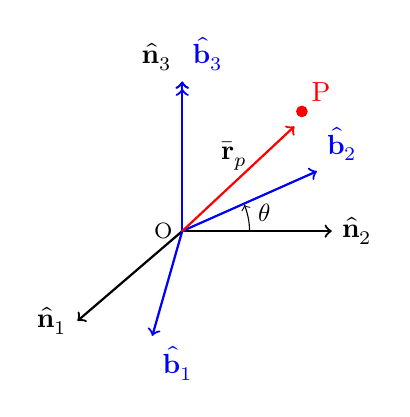
\begin{tikzpicture}[scale=0.95, line cap=round, line join=round]
        % origin
        \coordinate (O) at (0,0);
        \node at (O) [left] {\footnotesize$\text{O}$};

        % inertial (N) axes
        \draw[->, thick] (O) -- (-1.4,-1.2) node[left]  {$\hat{\mathbf n}_1$};
        \draw[->, thick] (O) -- ( 2.0, 0.0) node[right] {$\hat{\mathbf n}_2$};
        \draw[->, thick] (O) -- ( 0.0, 2.0) node[above left] {$\hat{\mathbf n}_3$};

        % body (B) axes
        \draw[->, thick, blue] (O) -- ( -0.4,-1.4) node[below right] {$\hat{\mathbf b}_1$};
        \draw[->, thick, blue] (O) -- ( 1.8, 0.8) node[above right] {$\hat{\mathbf b}_2$};
        \draw[->>, thick, blue] (O) -- ( 0.0, 2.0) node[above right] {$\hat{\mathbf b}_3$};

        % angle between b2 and n2
        \draw[->] (0.9,0.0) arc[start angle=0, end angle=23, radius=0.9];
        \node at (1.1,0.25) {\small$\theta$};

        % add vector r_p
        \draw[->, thick, red] (O) -- (1.5,1.4);
        \node at (1.0,1.0) [left] {$\bar{\mathbf r}_p$};
        % add point P at the end
        \filldraw[red] (1.6,1.6) circle (2pt) node[above right] {P};
    \end{tikzpicture}
\end{center}
\tagstructend

Let the position vector of point P be defined as:
\[
    \bar{\mathbf r}_p = x\,\hat{\mathbf b}_1 + y\,\hat{\mathbf b}_2 + z\,\hat{\mathbf b}_3
\]
In order to find the time derivative of $\bar{\mathbf r}_p$, we need to apply the product rule of differentiation:
\[
    \dot{\bar{\mathbf r}}_p = \dot{x}\,\hat{\mathbf b}_1 + x\,\dot{\hat{\mathbf b}}_1 + \dot{y}\,\hat{\mathbf b}_2 + y\,\dot{\hat{\mathbf b}}_2 + \dot{z}\,\hat{\mathbf b}_3 + z\,\dot{\hat{\mathbf b}}_3
\]

Now, let's consider that we have an observer in the frame $B$ and we want to express the velocity in the frame $B$. In this case, the time derivatives of the basis vectors are zero because they are fixed in frame $B$:
\[
    {}^{B} \dot{\bar{\mathbf r}}_p = \dot{x}\,\hat{\mathbf b}_1 + \dot{y}\,\hat{\mathbf b}_2 + \dot{z}\,\hat{\mathbf b}_3
\]

However, if the observer is in the frame $N$, the terms with the time derivatives of the basis vectors are not zero. Therefore, we need to use the Transport Theorem to find those terms:
\[
    {}^{N} \dot{\bar{\mathbf r}}_p = \dot{x}\,\hat{\mathbf b}_1 + x\,\dot{\hat{\mathbf b}}_1 + \dot{y}\,\hat{\mathbf b}_2 + y\,\dot{\hat{\mathbf b}}_2 + \dot{z}\,\hat{\mathbf b}_3 + z\,\dot{\hat{\mathbf b}}_3
\]
\[
    {}^{N} \dot{\bar{\mathbf r}}_p = \dot{x}\,\hat{\mathbf b}_1 + \dot{y}\,\hat{\mathbf b}_2 + \dot{z}\,\hat{\mathbf b}_3 + x\,(\bar{\boldsymbol{\omega}}_{B/N} \times \hat{\mathbf b}_1) + y\,(\bar{\boldsymbol{\omega}}_{B/N} \times \hat{\mathbf b}_2) + z\,(\bar{\boldsymbol{\omega}}_{B/N} \times \hat{\mathbf b}_3)
\]
This expression can be rewritten as:
\[
    {}^{N} \dot{\bar{\mathbf r}}_p = {}^{B} \dot{\bar{\mathbf r}}_p + \bar{\boldsymbol{\omega}}_{B/N} \times \bar{\mathbf r}_p
\]
and represents the inertial velocity of point P expressed in frame $B$ as observed from frame $N$.


\end{document}
